%%----------------------------------------------------------------------
%%----------------------------------------------------------------------
\clearpage
\pagetitle{Organization}

\begin{columns}

This section describes how to conduct a \emph{Legacies} campaign, and
is mostly intended for the organizer.

\missionheading{Schedule}

Recon Squad games can be easily run in about~60 minutes in an event
setting with boards pre-arranged and armies unpacked before the clock
starts for each round.  Generally matches take at most~90 minutes even
at a very casual pace with no preparation beforehand.  The Cataclysm
game can be comfortably played in~4 hours including setup.  It's
therefore feasible to run \emph{Legacies} over either several
evenings, or a single full day.  A sample schedule for a single-day is:

\bigskip
\centerline{\begin{tabular}{cl}
11:00	 	& Doors open\\
11:50	 	& Registration Closes\\
12:00	 	& Campaign Briefing \& Alliance Pairings\\
12:15	 	& Round 1\\
1:25	 	& Alliance Pairings\\
1:35	 	& Round 2\\
2:40	 	& Alliance Pairings\\
2:50	 	& Round 3\\
3:50	 	& Alliance Pairings\\
4:00	 	& Round 4\\
5:00	 	& Dinner Break\\
5:30	 	& The Cataclysm\\
9:30	 	& Campaign Outcome \& Prizes\\
\end{tabular}}

\vfill

\noindent\fbox{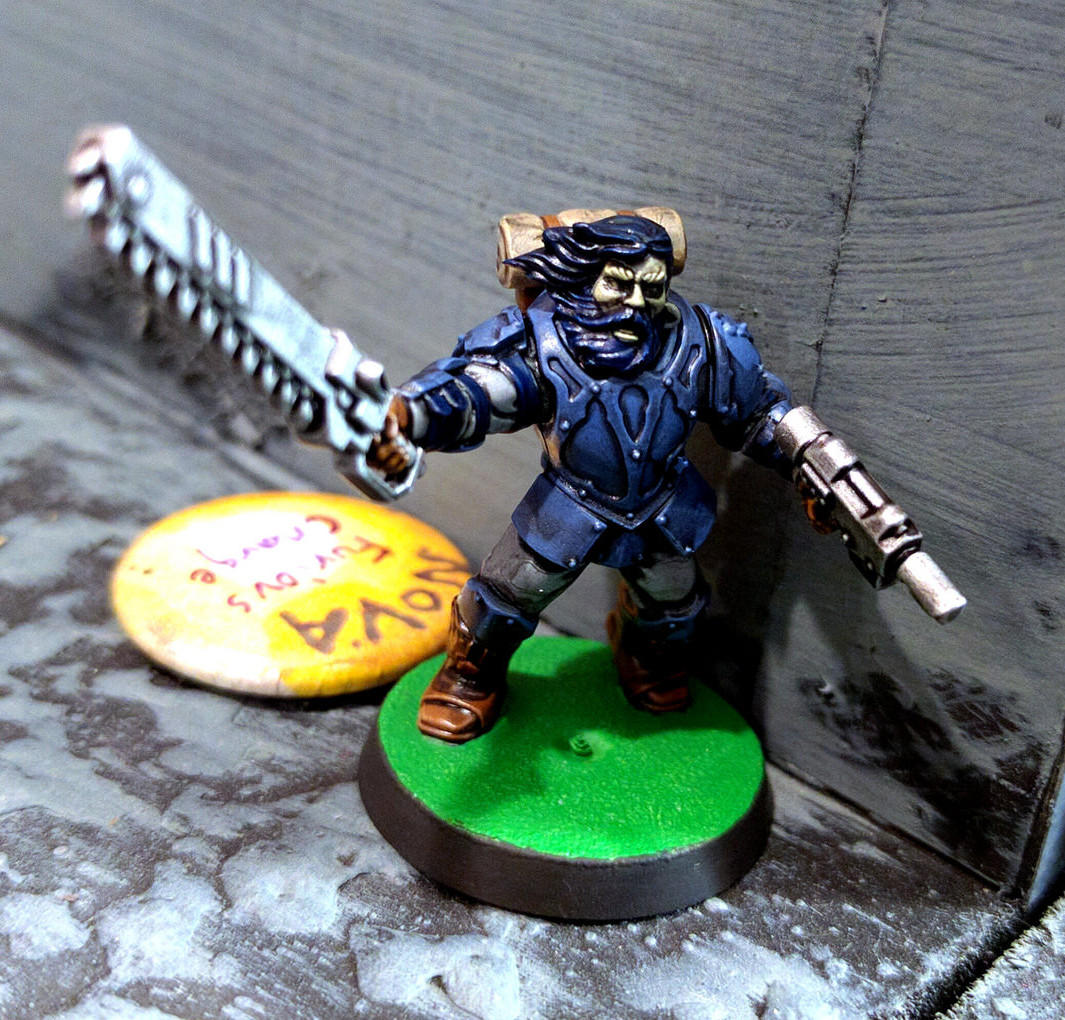
\includegraphics[width=\linewidth]{images/renegade-sgt-cropped.jpg}}

\columnbreak%

\missionheading{Alliances \& Story}

At the start of the campaign, the players are organized into two
alliances with an equal number of players.  In some groups this might
be faction specific, e.g., Chaos Daemons versus Eldar.  Generally
though an alliance will be comprised of several factions and can be
given a less specific title such as the Forces of Order, Legions of
Discord, or the Spoiler Horde.  How players are assigned alliances is
up to the organizer.  In a large event with mostly strangers and
tournament leanings it might be simply random.  In more
narrative-oriented and casual settings though, some attempt should be
made to take into account thematic cohesiveness as well as balanced
skill levels.

The concept behind the campaign is that each recon squad is a team of
veterans or other distinguished warriors tasked with several special
operations as part of a larger battle or war.  In the course of those
missions their paths eventually all cross, resulting in the larger
final battle.  Any specific background story is up to the organizer
and players, enabling a range of narratives with more or less detail.

\missionheading{Setup}

In advance of the campaign, players should at a minimum read the Recon
Squad rules and select their army list.  They should also be pointed
to the \emph{Legacies} Mission Pack, or this whole packet, in case
they wish to tailor their squad toward a particular legacy.

Preparing for the campaign is very simple.  For each of the two
alliances, print and cut apart enough sets of the~8 legacy cards at
the end of the Mission Pack section to have at least one card per
player.  Also print and cut apart enough sets of the~8 mission sheets
to have one for each match.  For a campaign with up to~16 players this
means making two sets of legacy cards and one set of mission sheets.

\missionheading{Legacies}

After being assigned an alliance, each player chooses a legacy.  No
legacy may be selected twice within an alliance until all legacies
have been chosen at least once, and so on if there are even more
players.  Otherwise the alliance members may discuss among themselves
how to divy up the legacies.  If there is any contention, either ask
the players in random order to choose, or randomly assign legacies.

Each legacy lists three Recon Squad Missions and gives a Cataclysm
Objective and Legacy Bonus.  To achieve their legacy, players must
accomplish the Cataclysm Objective in the final team battle.  If they
win at least two of the three Recon Squad Missions in the given role
of attacker, defender, or either, then they receive their Legacy Bonus
in the Cataclysm.

Players' chosen legacies, match results, and whether or not they are
succeeding at their missions are all public information throughout the
campaign.

\missionheading{Round Pairings}

Match pairings are made strategically by the alliances to help their
players achieve their legacy missions and further their collective
strategic goals.  Before each round, the alliances alternate
nominating one of their remaining unpaired players along with a
mission and role (attacker or defender).  The opposing alliance then
responds with a player for the match, who takes the other mission role
and chooses an unclaimed game board to play on.  This player must be
in the same or best similar win/draw/loss bracket as the nominated
player, unless the number of players is not great enough to make this
restriction without repeating match pairings.  In that case the later
rounds might require specific pairings to not have repeats.

For the first round, the initial alliance to put a player forward is
determined either randomly or based on the background story or the
outcomes of connected preceding events.  In subsequent rounds the
alliances alternate making the initial nomination.

Players should use the checkboxes on their legacy cards to record
victories toward the Recon Squad Mission requirements, in addition to
the organizer keeping track.  It does not matter if the player was
nominated or the responding opponent, and they do not have to complete
the missions in any order.  In order to get their Legacy Bonus in the
Cataclysm they simply have to win each mission in the required role at
some point in the campaign.  Similarly, a player can attempt a mission
and role pair multiple times.  However, no advantage is gained by
winning the same mission and role pair multiple times.

\missionheading{Cataclysm}

\missionheading{Scoring and Prizes}

\end{columns}
